\scanpage{4}
Localisant sur $Y$, on trouve
\[
 \underline{\operatorname{Ext}}^{\bullet}_{T'\deleted{\unsure{,Z'}},\,\unsure{\underline O_{U'}|\underline O_{X'}|\underline O_{\overline{X'}}}}
 (\overline{X'}/Y;\overline{F'},\overline{G'})
 \simeq\coprod_{n\in\mathbb Z}\underline{\operatorname{Ext}}^{\bullet}_{T\deleted{\unsure{\cap U}},\,\underline O_U}(X/Y;F,G(n))
\]
% slanted
\margin{N.B. \unsure{partir} \unsure{de modules|des modules} gradués,\ldots}
\[
 \deleted{\underline{\operatorname{Ext}}_{Z'\cap U'}}
\]
\deleted{D'autre part, on aura supposant pour simplifier $U=X$, donc $U'=X'$, $\overline{U'}=\overline{X'}$}
\[
 \deleted{\operatorname{Ext}^{\bullet}_{Z'\unsure{\cap U'},\,\underline O_{X'}}(X';F',G')
 \Longleftarrow H^p_{Z'}(X',\underline{\operatorname{Ext}}^q(F',G'\unsure{)\,)|\,}))}
\]
\figure{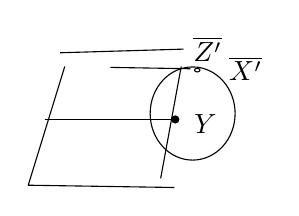
\begin{tikzpicture}[x=.58cm,y=.58cm]
 \draw (0,0)--(3.2,-.05) (0,0)--(.8,2.6) (2.9,.15)--(3.35,2.6);
 \draw (.7,2.9)--(3.4,2.98) node[right] {$\overline{Z'}$};
 \draw (1.8,2.58)--(3.55,2.55) (3.7,2.52) ellipse (.06 and .04);
 \draw (3.6,1.57) ellipse (.93 and 1.02);
 \draw (.36,1.44)--(3.22,1.44); \fill (3.22,1.44) circle (.09);
 \node at (3.88,1.35) {$Y$}; \node at (4.76,2.55) {$\overline{X'}$};
\end{tikzpicture}}
\figure{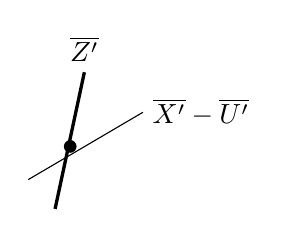
\begin{tikzpicture}[scale=.62]
 \draw[very thick] (.55,-1.3)--(1.15,1.5) node[above] {$\overline{Z'}$};
 \draw (0,-.7)--(2.35,.68) node[right] {$\overline{X'}-\overline{U'}$}; \fill (.86,-.02) circle (.13);
\end{tikzpicture}}
\diagram{\begin{tikzcd}[ampersand replacement=\&,row sep=small]
 \operatorname{Ext}^{\bullet}_{\overline{T'}\deleted{\unsure{,Z'}}}(\overline{X'};\overline{F'},\overline{G'})\\
 \operatorname{Ext}^{\bullet}_{\widehat{T'}}(\widehat{X'};\widehat{F'},\widehat{G'})\arrow[u]
\end{tikzcd}}
\figure{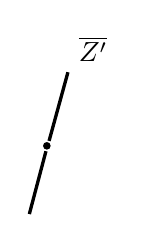
\begin{tikzpicture}[scale=.57]
 \draw[very thick] (.2,-1.5)--(.57,-.1) (.64,.13)--(1.06,1.66) node[above right] {$\overline{Z'}$}; \fill (.59,.02) circle (.085);
\end{tikzpicture}}
\[
 \underline H^p\bigl(\overline{Z'}\underset{\unsure{?}}{-}\overline{R'},
 \overbrace{\underline{\operatorname{Ext}}^{q}_{\overline{Z'}}(\overline{F'},\overline{G'})}\bigr)
\]
\margin{formation de ces \unsure{invariants} est compatible aux extensions plates de la base\ldots}
\figure{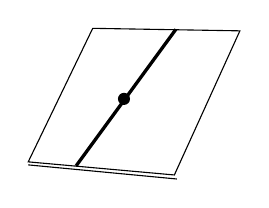
\begin{tikzpicture}[scale=.64]
 \draw (0,0)--(2.9,-.26)--(4.2,2.6)--(1.28,2.65)--cycle;
 \draw (0,-.06)--(2.95,-.34); \draw[very thick] (.95,-.08)--(2.93,2.63); \fill (1.9,1.25) circle (.12);
\end{tikzpicture}}
\[
 H^p(\overline{Z'}-\overline{R'},\overline E)
 \mathrel{\overset{\unsure{?|2}}{\underset{\longleftrightarrow}{\sim}}}
 H^p(\widehat{Z'}-\widehat{R'},\widehat E)
\]
\margin{\deleted{\unsure{par hypothèse|bij.-bij.}} \unsure{par localisé|pour localisé|par localis.}}
Le lemme des cinq nous ramène au cas des $H^p_{\overline{Z'}}(\overline{R'},\overline E)$, ou en changeant de \unsure{notations|notation} les $H^p_{\overline{Z'}}(\overline{X'},\overline E)$
\figure{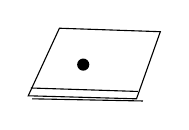
\begin{tikzpicture}[scale=.55]
 \draw (0,0)--(2.5,-.07)--(3.05,1.48)--(.72,1.56)--cycle;
 \draw (.06,.18)--(2.53,.1) (.09,-.07)--(2.65,-.12); \fill (1.27,.72) circle (.14);
\end{tikzpicture}}
\deleted{Mais ceci est} \unsure{Dégager|D'après|Dégageons} un \uline{lemme} sur les \unsure{changemts|changements} de base \uuline{plats} et \uuline{affines} sur les $\underline{\operatorname{Ext}}^{\unsure{\bullet|+}}_T(U;F,G)$.
% archive sheet number: 3

